\documentclass{fetch-my-doc}
\usepackage{tabu}
%\usepackage{multirow}
\usepackage{siunitx}
%\usepackage{enumitem}
%\usepackage{fancyvrb}
%\usepackage{breakurl}
%\usepackage{tocloft}
%\usepackage{pdflscape}
%\usepackage{ltxtable}
%\usepackage{filecontents}
\usepackage{onimage}

\sisetup{output-decimal-marker = {,}}

\definecolor{darkgreen}{rgb}{0,.5,0}

\hypersetup{breaklinks,colorlinks=true,citecolor=darkgreen,urlcolor=blue,linkcolor=blue,anchorcolor=blue} %,pdftex=true}

\newcommand{\hypref}[1]{\SaveVerb{myverb}|#1|\hyperlink{#1}{\protect\UseVerb{myverb}}}

\newcommand{\sep}{\begin{center}\noindent\rule{.5\textwidth}{0.5pt}\end{center}}

\newcommand{\rc}{\rowcolor{lightgray!40}}
\newcommand{\cc}{\columncolor{lightgray!40}}

\makeatletter
\newcommand*{\shift}[2]{%
  \settowidth{\@tempdima}{#2}%
  \makebox[\@tempdima]{\hspace*{#1}#2}%
}
\makeatother

% Linebreak nach paragraph
\makeatletter
\renewcommand\paragraph{%
   \@startsection{paragraph}{4}{0mm}%
      {-\baselineskip}%
      {.5\baselineskip}%
      {\normalfont\normalsize\bfseries}}
\makeatother

\def\imagetop#1{\raisebox{2.5em}{\vtop{\null\hbox{#1}}}}

%\renewcommand{\datum}{14.10.2012}
\renewcommand{\datum}{\today}
\renewcommand{\abgabe}{14.07.2014}
\renewcommand{\version}{1.0.0}
	%	Versionierung:
	%	x.y.z
	%	- x hoch bei ?
	%	- y hoch bei größeren Änderungen von ganzen Absätzen.
	%	- z hoch bei kleinen Verbesserungen wie Rechtschreibung, Satzbau, usw.
\renewcommand{\typ}{Dokumentation}
\renewcommand{\titel}{Dokumentation}
\renewcommand{\libdir}{./}
\bibliography{referenzen}

\setcounter{tocdepth}{4}
\setcounter{secnumdepth}{3}

\tikzset{
    image label/.style={
        every node/.style={
            fill=white,
            fill opacity=.5,
            text opacity=1,
            text=orange,
            font=\fontfamily{phv}\selectfont\Large\bfseries}
        }
}

\begin{document}
	\sloppy
	\begin{titlepage}
	\begin{center}
		\vspace*{.7cm}		
		\thispagestyle{FirstPage}
		\textsc{\LARGE \fach}\\
		%\vspace*{.2cm}
		%{\huge Fetch my ball}\\[0.4cm]
		
		
\includegraphics[width=0.85\textwidth]{\libdir img/logo1.pdf}\\
		%\textsc{\Large \gruppe}\\[0.5cm]

		% Titel
		\HRule \\[0.4cm]
		{ \huge \bfseries \titel}\\[0.4cm]
		Version \version	\\
		\HRule \\[1.5cm]

		\vfill
		
		% Autoren
		\begin{tabular}{rcl}
			\toprule
			\mgEinsVorname\ \mgEinsNachname		&&	\mgEinsMail	\\
			\mgZweiVorname\ \mgZweiNachname		&&	\mgZweiMail	\\
			\mgDreiVorname\ \mgDreiNachname		&&	\mgDreiMail	\\
			\bottomrule
		\end{tabular}
		
		\vspace{2cm}

		{\large Abgabe: \abgabe}
	\end{center}
	\addtolength{\textheight}{\versch}
\end{titlepage}
	\addtolength{\textheight}{\versch}
	%%%%%%%%%%%%%%%%%%%%%%%%%%%%%%%%%%%%
	% TODOS ENTFERNEN NICHT VERGESSEN! %
	%%%%%%%%%%%%%%%%%%%%%%%%%%%%%%%%%%%%
	\printtodo
	%%%%%%%%%%%%%%%%%%%%%%%%%%%%%%%%%%%%
	\addtocontents{toc}{\protect\sloppy}
	\tableofcontents
	\clearpage
	
	%\section{Versions- und Änderungsgeschichte}\label{sec:versionsaenderung}
		%\begin{tabularx}{\textwidth}{ccX}
			%\toprule
			%Version			&	Datum						&	Änderungen	\\\midrule
			%1.0.0				&	14.07.2014			&	Erste veröffentlichte Version	\\
			%\bottomrule
		%\end{tabularx}	
		%\clearpage
	
	\rowcolors*{0}{}{lightgray!40}
	
	%%%%%%%%%% Hier beginnt das Dokument %%%%%%%%%%
	\section{Einführung}\label{sec:Einfuehrung}
		\autor{...}

  \section{Technischer Aufbau}\label{sec:Aufbau}
		\autor{...}
    Unser Roboter wurde wie in der Aufgabenstellung beschrieben mittels der Lego NXT-Plattform, dem ROS-Framework und Common Lisp betrieben. Auf dem Roboter selber lief hierbei nur der NXT. Das Steuerprogramm wurde einem Rechner ausgeführt, welcher mittels USB-Schnittstelle mit dem NXT-Baustein kommunizieren konnte. Für die Schnittstelle zu ROS wurde das Paket NXT-ROS verwendet.

  Am Roboter befinden sich zwei verschiedene Sensoren: Ein Ultraschall-Sensor (d) mit Ausrichtung nach vorne und ein RGB-Farbsensor (c) mit Ausrichtung nach unten. Des weiteren verfügt der Roboter über drei Motoren, von denen zwei für die Steuerung der beiden Hinterräder zuständig sind (a, b), und einer den Gripper kontrolliert (e).
    
    \begin{center}
      \begin{minipage}[t]{.49\textwidth}
        \begin{figure}[H]%
          \centering%
          \caption{Die erste Version des Balls}%
          \label{}%
          \includegraphics[width=\columnwidth]{img/ball1.jpg}%
        \end{figure}
      \end{minipage}
      \hfill
      \begin{minipage}[t]{.49\textwidth}
        \begin{figure}[H]%
          \centering%
          \caption{Die finale Version des Balls}%
          \label{}%
          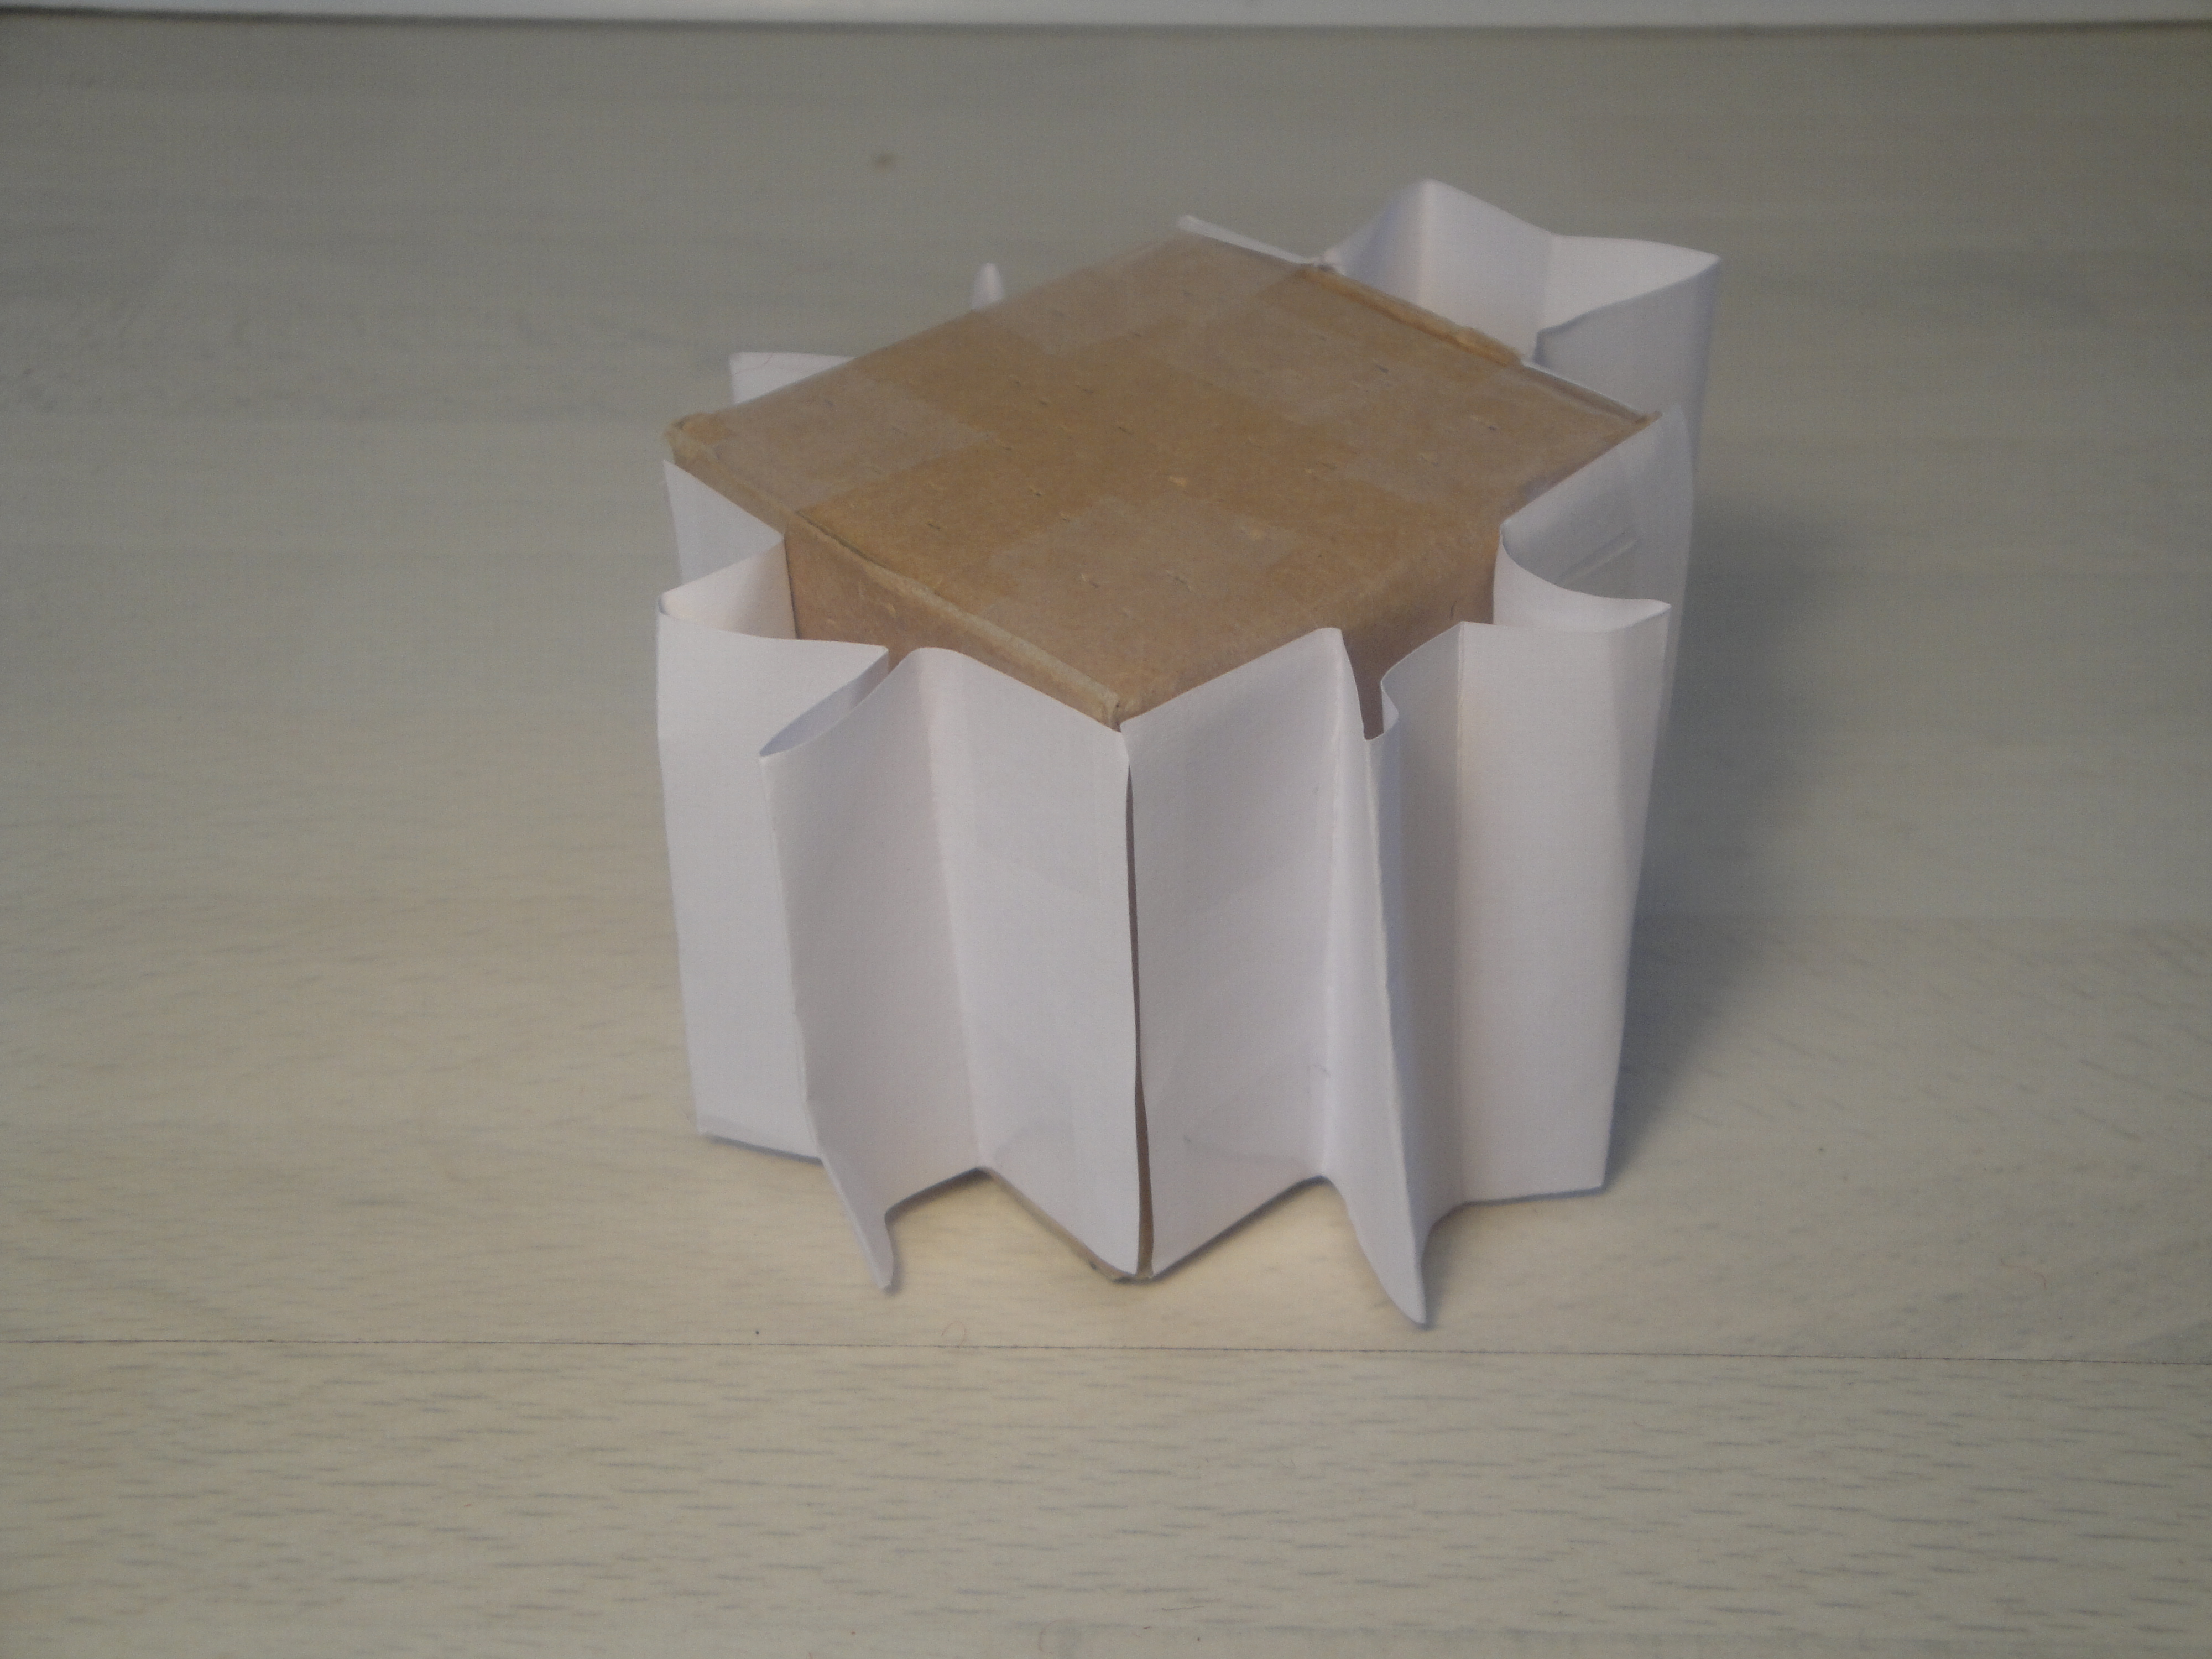
\includegraphics[width=\columnwidth]{img/ball2.jpg}%
        \end{figure}
      \end{minipage}
    \end{center}
    
    \begin{figure}[H]%
      \centering%
      \caption{blbla}%
      \label{}%
      \begin{tikzonimage}[width=\textwidth]{img/robbyOpenSideTop.jpg}[image label]
        \draw [orange, line width=3pt] (0.52,0.37) circle [radius=0.8cm] node [xshift=-1.25cm] {c};
        \draw [orange, line width=3pt] (0.835,0.23) circle [x radius=1.0cm, y radius=1.55cm] node [xshift=-1.5cm] {d};
        \draw [orange, line width=3pt] (0.6,0.55) circle [x radius=1.55cm, y radius=1.1cm] node [xshift=-1.5cm] {e};
      \end{tikzonimage}
    \end{figure}
    
    \begin{figure}[H]%
      \centering%
      \caption{blbla}%
      \label{}%
      \begin{tikzonimage}[width=\textwidth]{img/robbyOpenBottom.jpg}[image label]
        \draw [orange, line width=3pt] (0.4,0.39) circle [x radius=2.5cm, y radius=0.85cm] node [xshift=-2.95cm] {a};
        \draw [orange, line width=3pt] (0.4,0.56) circle [x radius=2.5cm, y radius=0.85cm] node [xshift=-2.95cm] {b};
        \draw [orange, line width=3pt] (0.66,0.485) circle [radius=0.8cm] node [xshift=-1.25cm] {c};
      \end{tikzonimage}
    \end{figure}
				
		
		\section{Zielsetzung}
		
			\subsection{Problemsituation}
			
			Die gegebene Problemsituation dieses Projektes war folgende: 
		
			In einem abgegrenzten Feld befindet sich ein Ball (oder etwas ähnliches). Das Feld hat einen dunklen Boden und ist von einem hellen Rand umgeben. Der Ball soll von dem Roboter gefunden, gegriffen und dann aus dem Feld befördert werden. Bevor der Roboter den Ball aus dem Feld befördert, soll er dieses nicht verlassen.
		
			\subsection{Ziele}
			
			Die oben beschriebene Situation sollte mithilfe der Umsetzung folgender Teilziele gelöst werden. 
			
				\begin{itemize}
					\item Der Roboter soll den Ball finden.
					\item Der Ball soll angefahren werden.
					\item Mithilfe des Greifers soll der Ball gegriffen werden.
					\item Der Ball soll aus dem Bereich transportiert werden.
					\item Ein überschreiten der weißen Fläche soll erkannt und darauf reagiert werden.
				\end{itemize}
				
			\subsection{Rahmenbedingungen}
				
			Damit keine Wände oder umliegende Gegenstände als Ball erkannt werden können, muss ein Bereich vom maximalen Durchmesser des Feldes, um dieses herum, frei sein.
			
		%\subsection{Referenzen}\label{sec:Referenzen}
			%Es folgt eine Auflistung aller Referenzen zu den im Architekturentwurf erwähnten Fremdressourcen und verwendeten Dokumenten.
				%\printbibliography[heading=none]
		%
		
	%\clearpage
	%\listoffigures
	
	%\listoftables
	%\clearpage
	%\appendix
	
\end{document}
